\documentclass[11pt]{article}

\usepackage{changepage}
\usepackage{graphicx}
\usepackage{amssymb} %math symbols
\usepackage{mathtools} %more math stuff
\usepackage{amsthm} %theorems, proofs and lemmas
\usepackage{optidef} %fast optimization problem notation
\usepackage{biblatex} %Imports biblatex package
\addbibresource{papers.bib} %Import the bibliography file

\usepackage{minted} % code highlighting

%% declaring abs so that it works nicely
\DeclarePairedDelimiter\abs{\lvert}{\rvert}%
\DeclarePairedDelimiter\norm{\lVert}{\rVert}%

\title{MICRO-453 - Boxfish robotics practical}
\author{Gabriel Vallat, Lucas Bost, Titouan Renard}

\begin{document}

\maketitle
\tableofcontents


\begin{figure}[h!]
    \centering
    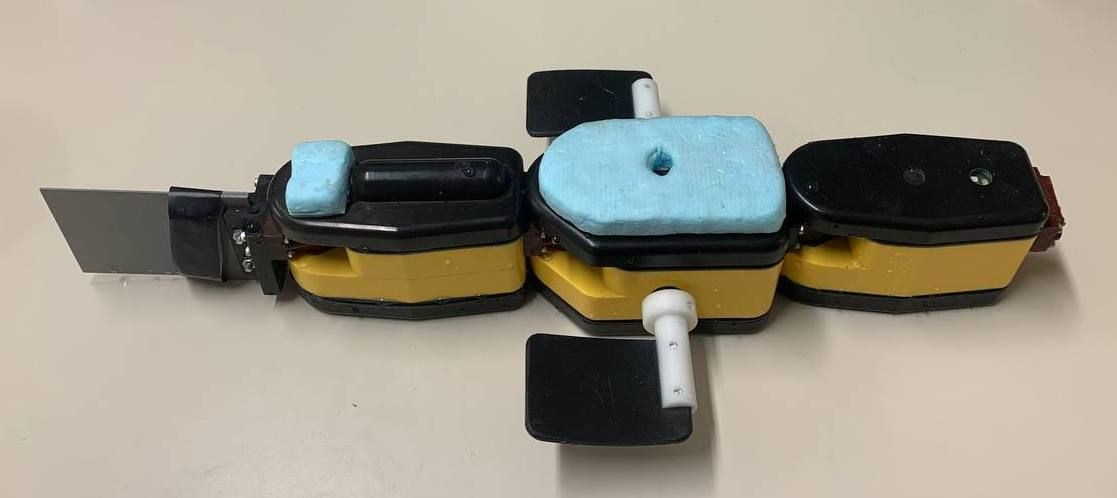
\includegraphics[width=\textwidth]{figures/side.jpg}
    \caption{Side view of the boxfish robot.}
    \label{boxfish}
\end{figure}


\section{Introduction and presentation of the hardware}

This report presents results from a practical session from the MICRO-453 course. It discusses the implementation of a simple control algorithm for a \textit{boxfish} bioinspired robot built out of \textit{salamadra robotica II} modules \cite{salamadra_robotica_2} (the robot is show in figure \ref{boxfish}). The robot is build of $3$ modules (a "head" a "body" and a "tail") and has $4$ actuated joints. The module configuration and the position of the actuated joints are displayed figure \ref{boxfish_labeled}. The head module contains a $32$-bits \textit{ARM7TDMI} micro-controller that be comunicated flashed remotely using a radio transmission setup. The PIC controller that implements the remote flashing of the head controller also allows for communication with the \textit{ARM7TDMI} over a radio channel. This enables the implementation of off-board logic on a separate computer. The modules are connected with each other using custom ports, they communicate over CAN busses and contain their own batteries. Each actuator is controlled using a PID control loop implemented on an separate micro-controller (one per actuator) and can be assigned a set-point by the head micro-controller. Furthermore each module has a RGB LED that can be used for debugging as well as localization of the robot in the testing environment.

\begin{figure}[h!]
    \centering
    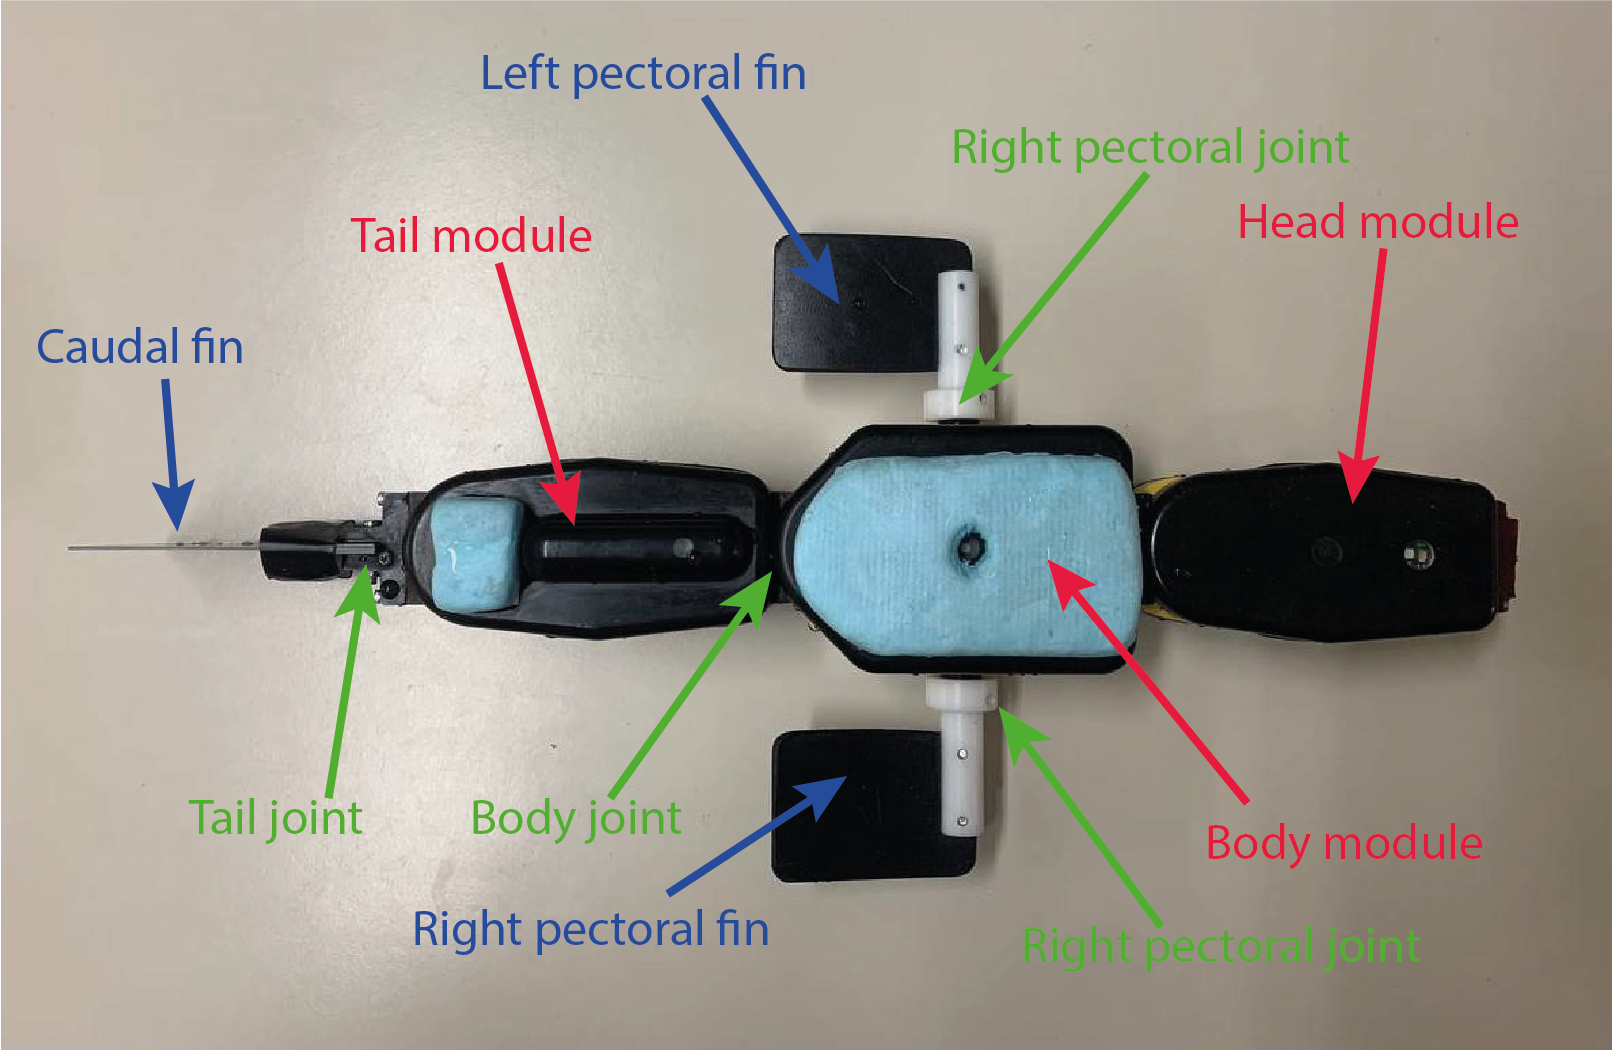
\includegraphics[width=\textwidth]{figures/top_annotated.png}
    \caption{Annotated top view of the boxfish robot.}
    \label{boxfish_labeled}
\end{figure}

\section{On-board and off-board software}

The software that is used for the control of the robot and that will be discussed in the report can be split up into \textit{on-board} software (the software that runs on the head \textit{ARM7TDMI} micro-controller and \textit{off-board} software (the software that runs on one of the laboratory's \textit{Windows} workstation). 
\\ \\
The \textit{on-board} software is written in C, compiled on \textit{Windows} and then sent over radio (using a custom radio interface on the workstation side and a dedicated micro-controller on the robot's side) to the robot where it is flashed on the \textit{ARM7TDMI} chip. 
\\ \\
The \textit{off-board} software is written in C++, compiled with \texttt{g++} and then runs directly on the \textit{Windows} workstation. The \texit{off-board} software communicates with the robot over radio but also interfaces over the local network with another workstation that handles tracking of the robot's position in the testing environment (this is discussed in more details in sub-section \ref{subsection:position_track}).
\subsection{Compiling and flashing the robot's microcontroller}

In the following section we discuss the compiling and flashing of the head ARM microcontroller as well as the first few tasks (points $1$ and $2$) that are asked for by the lab document.
\\ \\
The first program that we are asked to modify (point $1$ of the datum) changes the color of the LED in an infinite loop. It uses the function \texttt{set\_rgb(uint8\_t r, uint8\_t g, uint8\_t b)}, where r, g and b denote the intensities of the red, green and blue channels of an rgb led (the intensity values are between 0 and 127). In the example program the value of one color channel is changed every 10 ms (the delay is induced with the function \texttt{pause()}). %The LED first goes from extinct to red, then from red to yellow, from yellow to white, from white to cyan, from cyan to blue and from blue to extinct, and then it repeats this pattern. When we compile and run the program, the result is what we expected. 
To make the LED blink in green at 1 Hz, we change the content of the loop. We first light the LED in green setting the green channel to its max and red and blue to their min (\texttt{set\_rgb(0,127,0)}). And then we set every channel to their min values. To get a $1Hz$ frequency we simply set the pause time to $0.5s$ for both the on and off states of the LED (\texttt{pause(HALF\_SEC)}). %to set only the green channel. Then we write pause(HALF\_SEC) so that the light emits light during 0.5 second. And after we extinct the LED with \texttt{set\_rgb(0,0,0)} and the LED stays extinct during 0.5 second.
\\
\\
%The point $2$ of the datum requires us to provide an explanation of the display of the function \texttt{read\_registers()} called in ex2.cc. In \texttt{read\_registers()} there are some calls to the function \texttt{get\_reg\_b}, which consists of a read operation in the 8 bits registers. The first call is \texttt{regs.get\_reg\_b(6)}, so it will be a reading access in the 8-bits register of address 6. In the program main.c, in the register callback function it corresponds to a \texttt{ROP\_READ\_8} operation. In the switch, in the case \texttt{ROP\_READ\_8} at the address 6, we see that the value of the counter is assigned in \texttt{radio\_data}${\rightarrow}$\texttt{byte}, which is the value that is retrieved by the function \texttt{get\_reg\_b}. The value of the counter at the beginning is 0, so the value retrieved will be 0. In this case the counter is also set to 0 so here its value is unchanged. The second call is \texttt{regs.get\_reg\_b(21)} which corresponds in the switch to an operation \texttt{ROP\_READ\_8} at address 21. In this case a constant vaue of \texttt{0x42} is assigned in \texttt{radio\_data}${\rightarrow}$\texttt{byte} and the counter is incremented (i.e. counter = 1). The third call is once again \texttt{regs.get\_reg\_b(21)}, so the value that will be retrieved by the function is \texttt{0x42} and the counter will be incremented again (i.e. counter = 2). The fourth call is \texttt{regs.get\_reg\_b(6)}, so the value of the counter (counter = 2) will be retrieved and the counter is set back to 0. The last call is \texttt{regs.get\_reg\_b(6)}, so the value that will be retrieved is 0.
%Then there is a call of \texttt{display\_multibyte\_register(reg, 2)}. In this function, the program tries to read the content of the multibyte register of address 2 (\texttt{get\_reg\_mb()}). It displays the size of the buffer that is read (content of radio\_data${\rightarrow}$multibyte.size) and the content of the buffer (\texttt{radio\_data${\rightarrow}$multibyte.data[]}). In main.c, the function \texttt{get\_reg\_mb} at address 2 corresponds to the operation \texttt{ROP\_READ\_MB} at the address 2. In this case the variable \texttt{last\_mb\_size} is stored into \texttt{radio\_data}${\rightarrow}$\texttt{multibyte.size} and the variable \texttt{mb\_buffer[]} is stored into \texttt{radio\_data}${\rightarrow}$\texttt{multibyte.data[]}. At the beginning, \texttt{last\_mb\_size} is equal to 0 and there is nothing in \texttt{mb\_buffer} so the display will just be the size of the buffer which is 0. Then a buffer is created and the resulting buffer is: \texttt{[100,101,102,103,104,105,106,107]}. There is a call of \texttt{regs.set\_reg\_mb(2, buffer, sizeof(buffer)}, which corresponds to a writing operation in the multibyte of address 2. In \texttt{main.c} this is an operation \texttt{ROP\_WRITE\_MBWe} at address 2. In this case the content of \texttt{radio\_data}${\rightarrow}$\texttt{multibyte.size} is assigned to the variable \texttt{last\_mb\_size} and the content of \texttt{radio\_data}${\rightarrow}$\texttt{multibyte.data[]} is assigned into \texttt{mb\_buffer}, but every value of the buffer is incremented by 4. The value of \texttt{last\_mb\_size} is thus 8 and the content of the content of \texttt{mb\_buffer} is [104, 105, 106, 107, 108, 109, 110, 111]. Then there is a call of function \texttt{display\_multibyte\_register(regs, 2)}. In main.c it corresponds to an operation \texttt{ROP\_READ\_MB} at address 2. In this case the value of \texttt{last\_mb\_size} (it's equal to 8) is assigned in \texttt{radio\_data}${\rightarrow}$\texttt{multibyte.size} and the content of \texttt{mb\_buffer[]} is assigned in \texttt{radio\_data}${\rightarrow}$\texttt{multibyte.data[]} ([104,105,106,107,108,109,110,111]) and the display will be the size of the buffer and the buffer itself. Then there's a call set\_reg\_b(2, 11) which corresponds to a \texttt{ROP\_WRITE\_8} operation at address 2. In this case the first value of \texttt{mb\_buffer} is replaced by the value stored in \texttt{radio\_data}${\rightarrow}$\texttt{byte} which is equal to 11. For the call \texttt{set\_reg\_b(3, 22)} it's quite the same but the address is 3 and this is the second element of \texttt{mb\_buffer} that is replaced by the value contained in radio\_data${\rightarrow}$byte which is equal to 22. Then comes another call of \texttt{display\_multibyte\_register} so the display will be the size of the buffer (which hasn't changed) and \texttt{mb\_buffer} ([11,22,106,107,108,109,110,111]). Then we have a call of function \texttt{regs.set\_reg\_w(7,2121)} which corresponds in main.c to an operation \texttt{ROP\_WRITE\_16} (writing in 16 bits registers) at address 7. In the switch, in this case the value of a variable \texttt{datavar} is multiplied by 3 and incremented by the value stored in \texttt{radio\_data}${\rightarrow}$\texttt{word}. At the beginning the value of \texttt{datavar} is 0 and here the value contained in \texttt{radio\_data}${\rightarrow}$\texttt{word} is 2121 so the new value of \texttt{datavar} will be: ${3\times0 + 2121 = 2121}$. Then with \texttt{regs.get\_reg\_dw(2)} the program performs a reading operation in 32-bits registers. In the switch this corresponds to an operation \texttt{ROP\_READ\_32} at address 2. In this case the value of \texttt{datavar} is assigned in \texttt{radio\_data}${\rightarrow}$\texttt{word} and the display is the value of \texttt{datavar}. Then with the call \texttt{regs.set\_reg\_w(7,1765)} the new value of \texttt{datavar} is ${3\times2121 + 1765 = 8128}$. And finally with the last call of \texttt{regs.get\_reg\_dw(2)}, the new value of \texttt{datavar} is displayed. So the predicted display is:

The point $2$ of the datum requires us to provide an explanation of the display of the function \texttt{read\_registers()} called in ex2.cc. This function calls \texttt{get\_reg\_b}, \texttt{get\_reg\_w}, \texttt{get\_reg\_dw} and \texttt{get\_reg\_mb}, which consists in principle of a read operation in the 8, 16, 32 and multi bits registers respectively, as well as \texttt{set\_reg\_b}, \texttt{set\_reg\_w},\texttt{set\_reg\_dw} and  \texttt{set\_reg\_mb}, which are the set their respective set functions. Each of these functions are using the radio to communicate with the robot, and are accessing the registers via the same \texttt{register\_handler} callback function. In it, a switch is used to do custom operations, that are described below. 

\begin{itemize}
    \item \texttt{get\_reg\_b(6)}: return the value of \texttt{counter} (initialized at 0) then reset it
    \item \texttt{get\_reg\_b(21)}: increment \texttt{counter} and return 0x42 (or 66 in decimal)
    \item \texttt{get\_reg\_dw(2)} return \texttt{datavar}
    \item \texttt{get\_reg\_mb(2)}: return a word of the size of the last one written with \texttt{set\_reg\_mb(2)} (initialized as 0 byte)
    \item \texttt{set\_reg\_b(x,data)}: if $2\leq x \leq 4$, write data in the x-2 byte of the buffer used by \texttt{get\_reg\_mb(2)}
    \item \texttt{set\_reg\_mb(2,data[len],len)}: add 4 to each byte of data and write the result in the buffer used by \texttt{get\_reg\_mb(2)}
    
    \item \texttt{set\_reg\_w(7,data)}: multiply \texttt{datavar} (initialized at 0) by 3 and then add data.
\end{itemize}

Now that the functions are described, the output print of ex2 is quite easy to predict:

\begin{minted}{c}
get_reg_b(6) = 0 
get_reg_b(21) = 66
get_reg_b(21) = 66
get_reg_b(6) = 2
get_reg_b(6) = 0
get_reg_mb(2) = 0 // bytes:
get_reg_mb(2) = 8 // bytes: 104, 105, 106, 107, 108, 109, 110, 111
get_reg_mb(2) = 8 // bytes: 11, 22, 106, 107, 108, 109, 110, 111
get_reg_dw(2) = 2121
get_reg_dw(2) = 8128
\end{minted}

When we compile the program and run it, the result is the same as expected.



\subsection{Internal communication between the robot's modules}

In this part, in the main.c a body module (motor) is initialized. It uses the function of the CAN to store in a variable pos (signed integer on 8 bits) the value that is contained in the CAN register of address \texttt{MREG\_POSITION} in the module of address \texttt{MOTOR\_ADDR} with the function \texttt{bus\_get(MOTOR\_ADDR, MREG\_POSITION)}. This value is just the position of the actuator of address \texttt{MOTOR\_ADDR}. It uses the function \texttt{set\_rgb} to lights a LED in different color ranges depending on the sign of the position and the value of the position itself. When we compile the program and run it, we observe that the color of the LED is changing when we move the actuator by hand.
\\
\\
In order to get back continuously the position of the 4 actuators of the boxfish, we need to do several things. We first need to create a c++ file to be able to read values that are sent by radio from the robot to the computer. This program is quite similar to ex2.cc. We keep the function display\_multibyte\_register and only modify it a little bit so that the display is "Body dof, limb first dof, limb second dof and limb third dof positions are respectively: pos1, pos2, pos3, pos4". In the main function, we just add an infinite loop where we call the function display\_multibyte\_register and we choose address 0 that is free. In the main.c file, we add a constant BUFFER\_SIZE, which is the size of the buffer containing the positions and a static variable mb\_buffer[BUFFER\_SIZE] of type int8\_t which will contain the positions. We also have 4 const of type uint8\_t for the addresses of the 4 actuators. We add a register handler function as for exercise 2. In this function for a reading operation on multibytes registers at address 0, we assign the BUFFER\_SIZE in radio\_data${\rightarrow}$multibyte.size and mb\_buffer[] in radio\_data${\rightarrow}$multibyte.data[]. This allows to send the value of the positions to the computer. In the main function we register the register callback function with:



\begin{minted}{c}
radio_reg_add_callback(register_handler);
\end{minted}

And in the infinite loop of the main we use the CAN functions to retrieve the positions of the 4 actuators:

\begin{minted}{c}
//Gets the positions of all DOF
mb_buffer[0] = bus_get(BODY_DOF_ADR, MREG_POSITION);
mb_buffer[1] = bus_get(LIMB_DOF_1_ADDR, MREG_POSITION);
mb_buffer[2] = bus_get(LIMB_DOF_2_ADDR, MREG_POSITION);
mb_buffer[3] = bus_get(LIMB_DOF_3_ADDR, MREG_POSITION);
\end{minted}

\subsection{Robot-computer radio communication}
\label{subsection:radio}

In this part we send control inputs to an actuator (the tail joint actuator) directly over the radio channel from the workstation. We write a C++ program that generates and sends a wave function to the actuator (it remotely updates the set-point of the PID). In the main function of this program we declare a variable int \texttt{set\_val}. We wait the user to enter the mode (0 or 1) with:
\begin{minted}{c++}
cin << set_val;
\end{minted}
In an infinite loop, we write the value entered by the user using \texttt{regs.set\_reg\_b} at address \texttt{REG8\_MODE}. We don't need a register callback function because we use the 8 bits register bank which is handled by the system.
\\
\\
In order to send a sine wave by radio we modify a little bit the c++ program. Before the while loop we use \texttt{regs.set\_reg\_b(REG8\_MODE, 1)} to enter the demo mode (we could also wait the user to enter the mode). In the while loop we store a sine wave using the expression ${Asin(2{\pi}ft)}$ in a variable \texttt{set\_val} of type int, where A is the magnitude and f the frequency of the wave. In the code this is given by:
\begin{minted}{c++}
set_val = A*sin(2*M_PI*time_d()); //(for 1 Hz)
\end{minted}
Then we use \texttt{set\_reg} to write the value of the wave to a 8 bit register of address 1 (which is free). In the \texttt{main.c} file, we write register handler function that store the content of this register in a static variable and we use a function \texttt{get\_wave()} to be able to catch its value outside of the file (we could also put the register callback function in the file \texttt{modes.c}). In modes.c we modified the loop on the \texttt{REG8\_MODE} register value so that we just send the setpoint to the actuator:
\begin{minted}{c++}
// where a = get_wave();
bus_set(MOTOR_ADDR, MREG_SETPOINT, DEG_TO_OUTPUT_BODY(a));
\end{minted}
When we compile the program and run it, we see that the tail is doing oscillations as expected, but sometimes the motor stop a little bit, and that's because we send the wave by radio and the robot can sometimes lose the transmission and thus lose some values of the wave.


\subsection{Position tracking}
\label{subsection:position_track}

\begin{figure}
    \centering
    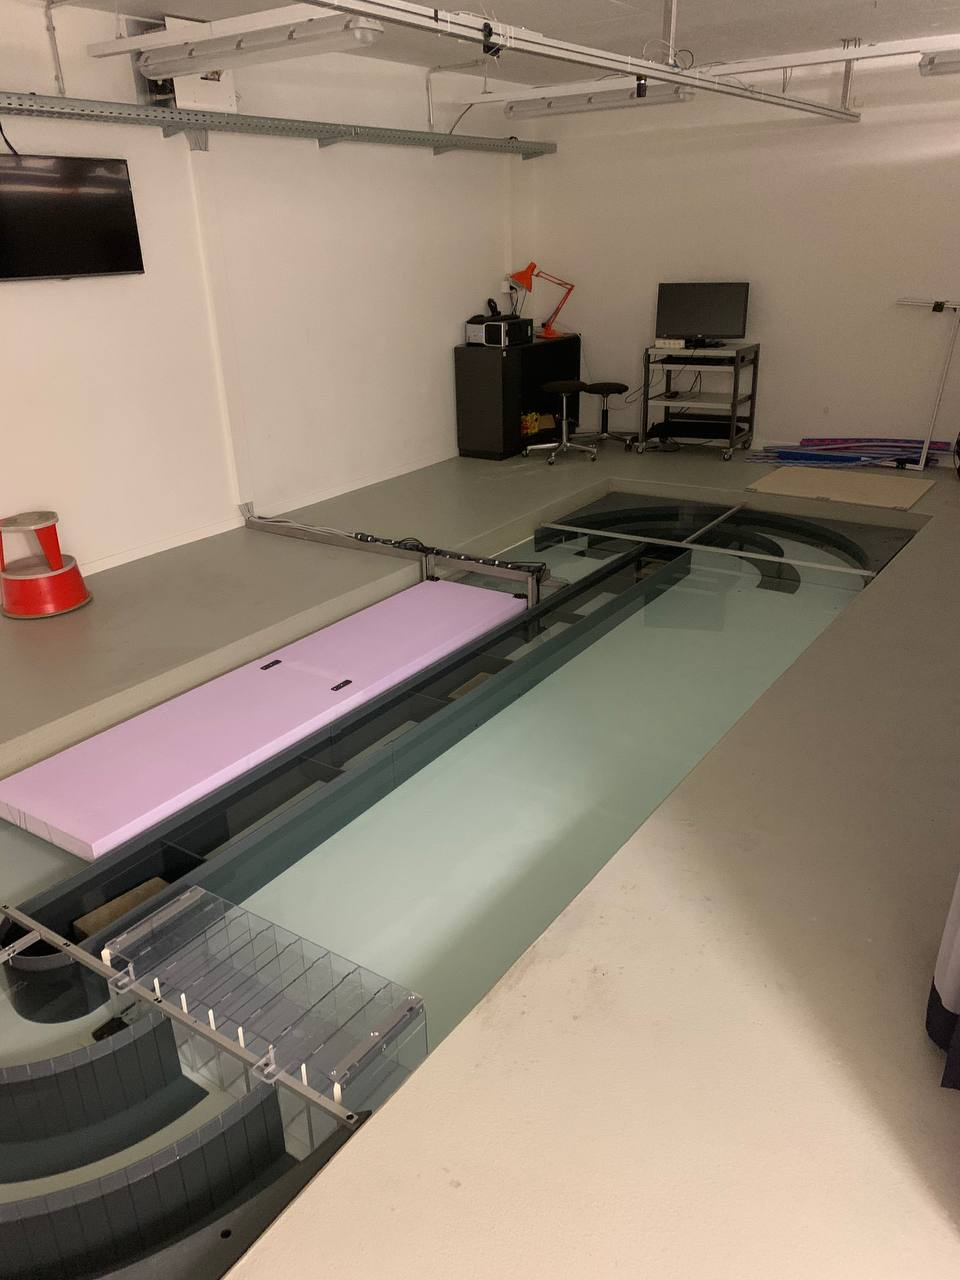
\includegraphics[width=0.4\textwidth]{figures/pool.jpg}
    \caption{The testing environment}
    \label{fig:basin}
\end{figure}

The testing environment a shallow $2 \times 6$ meter basin equipped with two ceiling mounted cameras that can be used to track the position of robots in the basin. The cameras give feedback to a lab computer that runs a simple spot-tracking algorithm, it is possible to access the position values (in the basin reference frame) by opening a TCP connection with the tracking PC over the lab's local network. Below we show a C++ code snippet from the reference file \texttt{ex6.cpp} that opens a TCP connection with the tracking PC and prints out the result in stdout.
\begin{minted}{c++}
// host name of the tracking PC
const char* TRACKING_PC_NAME = "biorobpc6";   

// port number of the tracking PC
const uint16_t TRACKING_PORT = 10502;          

int main()
{
  CTrackingClient trk;

  // Connects to the tracking server
  if (!trk.connect(TRACKING_PC_NAME, TRACKING_PORT)) {
    return 1;
  }

  while (!kbhit()) {
    uint32_t frame_time;
    // Gets the current position
    if (!trk.update(frame_time)) {
      return 1;
    }

    double x, y;
    cout.precision(2);
    
    // Gets the ID of the first spot
    // (the tracking system supports tracking multiple spots)
    int id = trk.get_first_id();
    
    // Reads its coordinates 
    // (if (id == -1), then no spot is detected)
    if (id != -1 && trk.get_pos(id, x, y)) {
      cout << "(" << fixed << x << ", " << y << ")" << " m \r";
    } else {
      cout << "(not detected)" << '\r';
    }
    
    // Waits 10 ms before getting the info next time 
    // (anyway the tracking runs at 15 fps)
    Sleep(10);
  }
\end{minted}
Using a dummy robot (a floater with a LED attached to it) and \texttt{ex6.cpp} we checked that the tracking system gives good read out and indeed we get good readouts. 
\\ \\
The point $6.1$ from the lab documents asks us to update the color of the LED as a function of robot's position in the basin, we therefore modify \texttt{ex6.cpp} so that it connects to robot over the radio channel (as in sub-section \ref{subsection:radio}) and we modify the tracking loop so that it updates the LED color. We make the red channel a function of the $x$ coordinate, and the blue channel a function of the $y$ coordinate. The green channel is kept at a high value $64$ to ensure the tracker continuously has a bright spot to track.

\begin{minted}{c++}
    r = ENCODE_PARAM_8(x,0,6);
    g = 64;
    b = ENCODE_PARAM_8(y,0,2);
    rgb = ((uint32_t)r << 16) | ((uint32_t)g << 8) | b; 

    regs.set_reg_dw(0,rgb);
\end{minted}
Manually moving the fish in the basin shows that indeed our system works and the color gets updated as expected.

\section{Control of the boxfish}

\subsection{Simple onboard, parametric trajectory generation}

In the datum, it was asked to change the amplitude of the wave to 40 and to send it to the actuator in the loop of sine\_demo\_mode function (5.1), but in our case, we directly implemented the parameters to be able to test other amplitudes and frequencies (5.2 of the datum). To do so we added two variables: \texttt{amp} and \texttt{freq} that could be entered in the terminal. Here are the modification that we did to the mode.c file that was provided:

To begin with, here is the register handler that we used. The \texttt{DECODE\_PARAM} macro is used to convert the message transmitted through the radio to a float with the maximum accuracy in the given range (that needed to be specified in both the sender and the receiver).
\begin{minted}{c}
static int8_t register_handler(uint8_t operation, uint8_t address,
                                RadioData* radio_data)
{
  uint8_t out;
  if(operation == ROP_WRITE_8)
  {
    if (address == 1) {
        out = radio_data->byte;
        freq = DECODE_PARAM_8(out,0,2);
        return TRUE;
      }
    if (address == 2) {
        out = radio_data->byte;
        amp = DECODE_PARAM_8(out,0,60);
        return TRUE;
      }
  }
  return FALSE;
}
\end{minted}
Once the parameters were recieved, the sine wave could then generated in the same way as for the LEDs, with the following modifications: The motors needed to be initialised by calling 
\begin{minted}{c}
  init_body_module(MOTOR_ADDR);
  start_pid(MOTOR_ADDR);
\end{minted}
The sine wave was created using our variables:
\begin{minted}{c}
  l = amp * sin(M_TWOPI * freq * my_time);
\end{minted}
And then outputed on the motor using:
\begin{minted}{c}
bus_set(MOTOR_ADDR, MREG_SETPOINT, DEG_TO_OUTPUT_BODY(l));
\end{minted}
One additional step was to needed to stop the motion when exiting the loop, which was done by writing 
\begin{minted}{c}
  bus_set(MOTOR_ADDR, MREG_SETPOINT, DEG_TO_OUTPUT_BODY(0.0));
  pause(ONE_SEC);
  bus_set(MOTOR_ADDR, MREG_MODE, MODE_IDLE);
\end{minted}
After the loop. We retrospectively noted that the motors should also be uninitialised at this moment. %OUPS lol

We also wrote a c++ program where the user enter the mode and our variables, whose value we stored the value in the register of addresses 1,2 and \texttt{REG8\_MODE}, using \texttt{regs.set\_reg()}. When we compiled the program and ran it, the strange behavior that was appearing when we send the wave by radio disappeared, as there was no more loss in transmission.

The c++ code is included in the joint file if you're interested in reading it. 

\subsection{Proposed swimming controller}

In order to generate a forward swimming motion of or our robot we propose the following swimming gait, described as follows. Let $\phi_1$ denote the angle of the body joint ($\phi_1 = 0$ when the the robot's tail modules is aligned with the body module), $\phi_2$ denotes the angle of the tail joint($\phi_1 = 0$ when the the tail module is aligned with the caudal fin). See figure \ref{boxfish_labeled} for a description of the position of joints on the robot. Let $\phi_3$ and $\phi_4$ denote the angles of both pectoral fins. Let : 
\begin{equation}
\label{swimming_trajectories}
\begin{aligned}
    \phi_1(t, \theta) = \alpha \left( cos(\omega t) \right) + \theta \cdot \alpha \gamma_1, \\
    \phi_2(t, \theta) = \alpha \beta \left( cos(\omega t) \right) + \theta \cdot \alpha \beta \gamma_1, \\
    \phi_3(t, \theta) = min(\gamma_2 \theta, 0),\\
    \phi_4(t, \theta) = min(-\gamma_2 \theta, 0).
\end{aligned}
\end{equation}
Where $\theta$ controls the turning rate, $\omega$ the undulation pulsation, $\alpha$ the undulation amplitude ($\beta$ is a scaling factor that allows for the caudal fin to undulate at a different amplitude than the tail module) and $\gamma_1, \gamma_2$ are gain parameters that modulate the response to turning rate input. The pectoral fins are used as differential breaks when turning. This controller is inspired by the limit-cycle behavior of a CPG controller on this robot as presented by Benjamin Frankenhauser in his semester project on the control of the boxybot robot \cite{boxybot_2}. 
\\
\\
We implement the trajectories described in (\ref{swimming_trajectories}) \textit{on-board}: 

\begin{minted}{c}
do {
    // Calculates the delta_t in seconds 
    //and adds it to the current time
    dt = getElapsedSysTICs(cycletimer);
    cycletimer = getSysTICs();
    delta_t = (float) dt / sysTICSperSEC;
    my_time += delta_t;

    // Calculates the sine wave
    body = alpha * (sin(M_TWOPI * freq * my_time) + 
           turn * gamma_1);
    tail = alpha * beta * (sin(M_TWOPI * freq * my_time)+ 
           turn * gamma_1 );
    left =  (turn<0)?    turn * gamma_2: 0;
    right = (turn > 0)?  turn * gamma_2: 0;

    // Outputs the sine wave to the motors
    bus_set(MOTOR_ADDR_BODY, MREG_SETPOINT, 
           DEG_TO_OUTPUT_BODY(body));
    bus_set(MOTOR_ADDR_TAIL, MREG_SETPOINT, 
           DEG_TO_OUTPUT_BODY(tail));
    bus_set(MOTOR_ADDR_LEFT, MREG_SETPOINT, 
           DEG_TO_OUTPUT_BODY(left));
    bus_set(MOTOR_ADDR_RIGHT, MREG_SETPOINT, 
           DEG_TO_OUTPUT_BODY(right));

    // Make sure there is some delay, 
    // so that the timer output is not zero
    pause(ONE_MS);

  } while (reg8_table[REG8_MODE] == IMODE_SINE_DEMO);
\end{minted}

We control the robot's behavior remotely by transmitting the swimming parameters $\theta$, $\omega$, $\alpha$, $\beta$, $\gamma_1$ and $\gamma_2$ as well as a \texttt{mode} flag that starts and stops the gait over radio from a C++ application. 
\\ \\
Experiments show that our controller is not only able to generate forward motion of the robot but also turning motion. We discuss and analyse the influence of $\omega$ and $\alpha$ on forward speed in sub-section \ref{experiments}.

\section{Experiment}

\subsection{Optimizing the swimming gait}
\label{experiments}
\begin{figure}
    \centering
    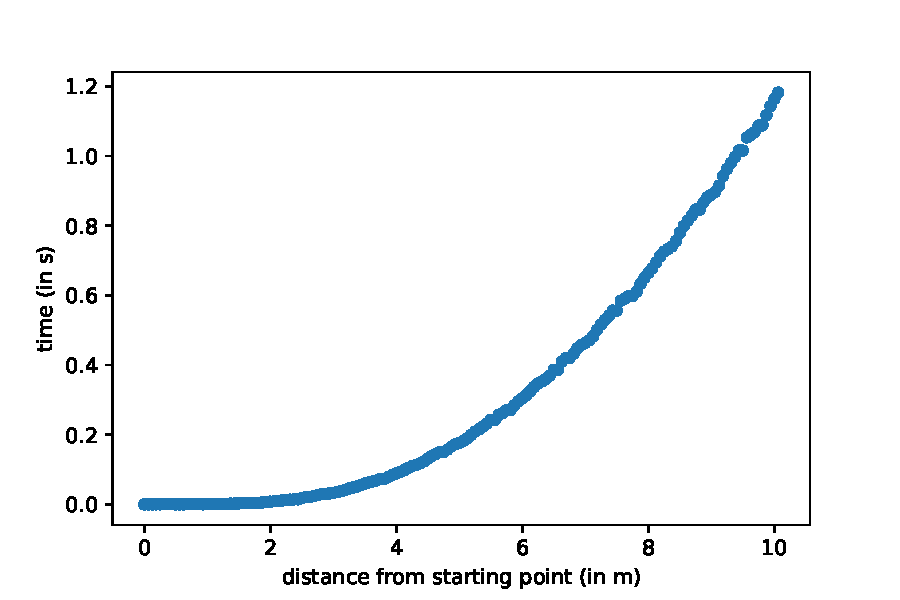
\includegraphics[width=0.8\textwidth]{figures/out-20-1_5-1.pdf}
    \caption{Plot of the distance (in $m$) versus time (in $s$) from the starting point as the robot starts it's gait. In this example the parameters are $\omega = 1$ and $\alpha = 20$.}
    \label{fig:trajectory_1}
\end{figure}
In order to better understand the influence of our parameters and optimize the swimming speed we propose to go through a rough grid search of the $\alpha$ and $\omega$ (amplitude and pulsation) space. To evaluate the swimming speed we make use of the tracking system presented in sub-section \ref{subsection:position_track}. 
\\ \\
The tracking system gives us position values (in the reference frame of the basin) over time. To evaluate speed we first compute the distance $d(t)$ from the position at time 0 :
\begin{align}
    d(t) = \norm{\vec{x}(t)-\vec{x}(0)}_2.
\end{align}
The evolution of distance $d(t)$ over time resembles the solution to a first order differential equation and converges to a constant terminal speed $v$ (as can be observed in figure \ref{fig:trajectory_1}). We compute an estimate $\hat{v}$ of $v$ by selecting a window at the end of the acceleration phase (where we consider the speed to be constant) and using linear regression to get a speed value. 
\\ \\
We fix the values :
\begin{align*}
	\theta = 0,\\
	\beta = 1,\\
	\gamma_1  = 5,\\
	\gamma_2 = 40.
\end{align*}
We search evaluate the terminal speed for every point $\vec{p}_{\omega,\alpha}$ in the space described by :
\begin{align*}
    \vec{p}_{\omega,\alpha} = (\omega, \alpha), \\
    \alpha \in \{ 10, 20, 30 \}, \\
    \omega \in \{ 1.0, 1.5, 2.0 \}. 
\end{align*}
For each point $\vec{p}_{\omega,\alpha}$ we run $3$ tests. We thus make a total of $27$ measurements. 



\begin{figure}
    \centering
    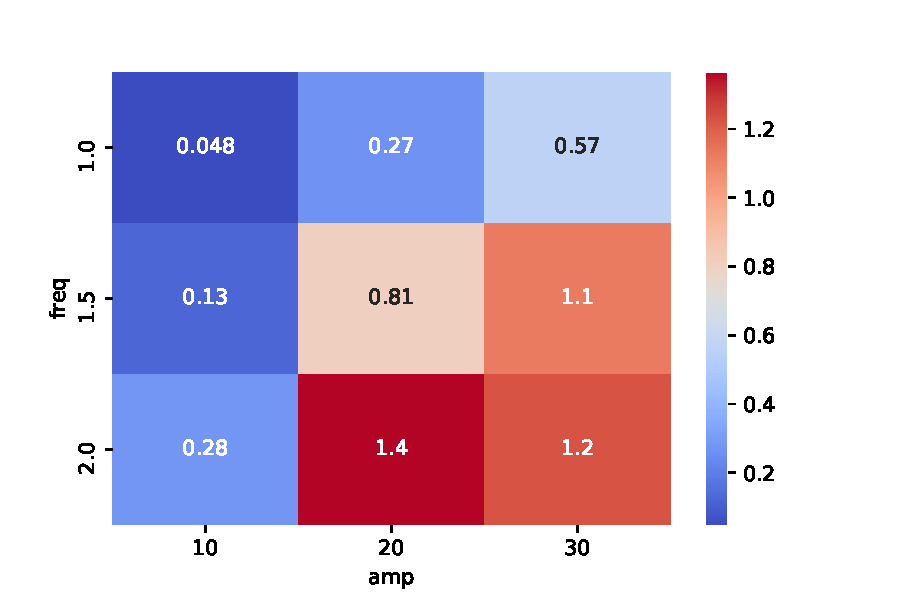
\includegraphics{figures/heatmap_speed.pdf}
    \caption{Heatmap representation of the speed (in $km/h$) as a function of oscillation frequency (in $Hz$) and amplitude (in degrees).}
    \label{fig:heatmap_speed}
\end{figure}
\\
\textit{TODO : analyser la heatmap, présenter la variance, noter les unités sur les graphes}
\\

\subsection{Optimizing the position controller}

\printbibliography %Prints bibliography

\end{document}
